% !TEX encoding = UTF-8 Unicode
% !TEX TS-program = xelatex 
\begin{QUESTIONS}
    \begin{QUESTION}
        \begin{ExamInfo}{098}{學測}{單選}{1}
        \end{ExamInfo}
        \begin{ExamAnsRateInfo}{85}{99}{95}{61}
        \end{ExamAnsRateInfo}
        \begin{QBODY}
			數列 $a_1 + a_2, \dots ,a_k +2k , \dots , a_{10} +20$ 共有十項,且其和為240,則 $a_1 + \cdots +a_k + \cdots +a_{10}$ 之值為 
			\begin{QOPS} 
				\QOP 31 
				\QOP 120 
				\QOP 130 
				\QOP 185	
				\QOP 218 。
			\end{QOPS}
        \end{QBODY}
        \begin{QFROMS}
        \end{QFROMS}
        \begin{QTAGS}\QTAG{B2C1數列級數}\end{QTAGS}
        \begin{QANS}
            (3)
        \end{QANS}
        \begin{QSOLLIST}
        \end{QSOLLIST}
        \begin{QEMPTYSPACE}
        \end{QEMPTYSPACE}
    \end{QUESTION}
    \begin{QUESTION}
        \begin{ExamInfo}{098}{學測}{單選}{2}
        \end{ExamInfo}
        \begin{ExamAnsRateInfo}{23}{36}{18}{15}
        \end{ExamAnsRateInfo}
        \begin{QBODY}
			令 $a = \cos (\pi^2 )$,試問下列哪一個選項是對的?
			\begin{QOPS} 
				\QOP $a= -1$
				\QOP $-1< a \leq -\frac{1}{2}$
				\QOP $-\frac{1}{2} < a \leq 0$ 
				\QOP $0 < a \leq \frac{1}{2}$ 
				\QOP $\frac{1}{2} < a \leq 1 $
			\end{QOPS}
        \end{QBODY}
        \begin{QFROMS}
        \end{QFROMS}
        \begin{QTAGS}\QTAG{B3C1三角}\end{QTAGS}
        \begin{QANS}
            (2)
        \end{QANS}
        \begin{QSOLLIST}
        \end{QSOLLIST}
        \begin{QEMPTYSPACE}
        \end{QEMPTYSPACE}
    \end{QUESTION}
    \begin{QUESTION}
        \begin{ExamInfo}{098}{學測}{單選}{3}
        \end{ExamInfo}
        \begin{ExamAnsRateInfo}{27}{39}{25}{17}
        \end{ExamAnsRateInfo}
        \begin{QBODY}
			已知 $f(x)$, $g(x)$ 是兩個實係數多項式,且知 $f(x)$ 除以 $g(x)$ 的餘式為 $x^4 -1$。試問下列哪一個選項不可能是 $f(x)$ 與 $g(x)$ 的公因式? 
			\begin{QOPS} 
				\QOP 5 
				\QOP $x-1$ 
				\QOP $x^2-1$ 
				\QOP $x^3-1$ 
				\QOP $x^4-1$
			\end{QOPS}
        \end{QBODY}
        \begin{QFROMS}
        \end{QFROMS}
        \begin{QTAGS}\QTAG{B1C2多項式函數}\end{QTAGS}
        \begin{QANS}
            (4)
        \end{QANS}
        \begin{QSOLLIST}
        \end{QSOLLIST}
        \begin{QEMPTYSPACE}
        \end{QEMPTYSPACE}
    \end{QUESTION}
    \begin{QUESTION}
        \begin{ExamInfo}{098}{學測}{單選}{4}
        \end{ExamInfo}
        \begin{ExamAnsRateInfo}{42}{80}{38}{8}
        \end{ExamAnsRateInfo}
        \begin{QBODY}
		甲、乙、丙三所高中的一年級分別有 3、4、5 個班級。從這 12 個班級中隨機選取一班參加國文抽考,再從未被抽中的 11 個班級中隨機選取一班參加英文抽考。則參加抽考的兩個班級在同一所學校的機率最接近以下哪個選項?
			\begin{QOPS} 
				\QOP 21 $\%$  
				\QOP 23$\%$ 
				\QOP $25\%$ 
				\QOP $27\%$  
				\QOP $29\%$
			\end{QOPS}
        \end{QBODY}
        \begin{QFROMS}
        \end{QFROMS}
        \begin{QTAGS}\QTAG{B2C3機率}\end{QTAGS}
        \begin{QANS}
            (5)
        \end{QANS}
        \begin{QSOLLIST}
        \end{QSOLLIST}
        \begin{QEMPTYSPACE}
        \end{QEMPTYSPACE}
    \end{QUESTION}
    \begin{QUESTION}
        \begin{ExamInfo}{098}{學測}{單選}{5}
        \end{ExamInfo}
        \begin{ExamAnsRateInfo}{50}{86}{47}{17}
        \end{ExamAnsRateInfo}
        \begin{QBODY}
			假設甲、乙、丙三鎮兩兩之間的距離皆為 20 公里。兩條筆直的公路交於丁鎮,其中之一通過甲、乙兩鎮而另一通過丙鎮。今在一比例精準的地圖上量得兩公路的夾角為 $45^\circ$,則丙、丁兩鎮間的距離約為 
			\begin{QOPS}
				\QOP 24.5 公里 
				\QOP 25 公里 
				\QOP 25.5 公里 
				\QOP 26 公里 
				\QOP 26.5 公里 
			\end{QOPS}
        \end{QBODY}
        \begin{QFROMS}
        \end{QFROMS}
        \begin{QTAGS}\QTAG{B3C1三角}\end{QTAGS}
        \begin{QANS}
            (1)
        \end{QANS}
        \begin{QSOLLIST}
        \end{QSOLLIST}
        \begin{QEMPTYSPACE}
        \end{QEMPTYSPACE}
    \end{QUESTION}
    \begin{QUESTION}
        \begin{ExamInfo}{098}{學測}{單選}{6}
        \end{ExamInfo}
        \begin{ExamAnsRateInfo}{33}{58}{27}{14}
        \end{ExamAnsRateInfo}
        \begin{QBODY}
			試問坐標平面上共有幾條直線,會使得點 $O(0,0)$ 到此直線之距離為 1,且點 $A(3,0)$ 到此直線之距離為 2?
			\begin{QOPS} 
				\QOP 1 條        
				\QOP 2 條 
				\QOP 3 條 
				\QOP 4 條 
				\QOP 無窮多條
			\end{QOPS}
        \end{QBODY}
        \begin{QFROMS}
        \end{QFROMS}
        \begin{QTAGS}\QTAG{B3C2直線與圓}\end{QTAGS}
        \begin{QANS}
            (3)
        \end{QANS}
        \begin{QSOLLIST}
        \end{QSOLLIST}
        \begin{QEMPTYSPACE}
        \end{QEMPTYSPACE}
    \end{QUESTION}
\end{QUESTIONS}
\begin{QUESTIONS}
    \begin{QUESTION}
        \begin{ExamInfo}{098}{學測}{多選}{7}
        \end{ExamInfo}
        \begin{ExamAnsRateInfo}{39}{67}{35}{15}
        \end{ExamAnsRateInfo}
        \begin{QBODY}
			試問下列哪些選項中的數是有理數? 
			\begin{QOPS} 
				\QOP $3.1416$
				\QOP $3$ 
				\QOP $\log_{10} \sqrt{5}+ \log_{10}\sqrt{2}$ 
				\QOP $\frac{\sin{15^\circ}}{\cos{15^\circ}} +  \frac{\cos{15^\circ}}{\sin{15^\circ°}}$ \quad 
				\QOP 方程式 $x^3 - 2x^2 +x-1=0$ 的唯一實根。
			\end{QOPS}
        \end{QBODY}
        \begin{QFROMS}
        \end{QFROMS}
        \begin{QTAGS}\QTAG{綜合}\end{QTAGS}
        \begin{QANS}
            (1)(3)(4)
        \end{QANS}
        \begin{QSOLLIST}
        \end{QSOLLIST}
        \begin{QEMPTYSPACE}
        \end{QEMPTYSPACE}
    \end{QUESTION}
    \begin{QUESTION}
        \begin{ExamInfo}{098}{學測}{多選}{8}
        \end{ExamInfo}
        \begin{ExamAnsRateInfo}{46}{80}{42}{16}
        \end{ExamAnsRateInfo}
        \begin{QBODY}
			如圖所示,正立方體 $ABCD - EFGH$ 的稜長等於 2 (即 $\overline{AB} = 2$ ), $K$ 為正方形 $ABCD $ 的中心,$M$, $N$ 分別為線段 $\overline{BF}$ ,  $\overline{EF}$ 的中點。試問下列哪些選項是正確的? 
			\begin{QOPS} 
				\QOP  $\lvec{KM} = \frac{1}{2} \lvec{AB} - \frac{1}{2} \lvec{AD} + \frac{1}{2} \lvec{AE}$ 
				\QOP $\lvec{KM} \cdot \lvec{AB}=1$ 
				\QOP $\lvec{KM}=3$ 
				\QOP  $\triangle KMN$ 為一直角三角形 
				\QOP $\triangle KMN$ 之面積為 $\frac{\sqrt{10}}{2}$。
			\end{QOPS}
			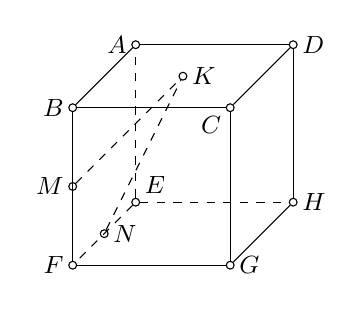
\begin{tikzpicture}
				\begin{scope}
				\small
				\tikzstyle{vnode}=[draw,circle,inner sep =1pt];
				\node[vnode] (v000) at (0,0) {};
				\node[anchor =south west] (t000) at (v000) {$E$};
				\node[vnode] (v001) at (0,2) {$$};
				\node[anchor =east] (t000) at (v001) {$A$};
				\node[vnode] (v011) at (2,2) {$$};
				\node[anchor =west] (t011) at (v011) {$D$};
				\node[vnode] (v010) at (2,0) {$$};
				\node[anchor =west] (t010) at (v010) {$H$};
				\node[vnode] (v100) at (-.8,-.8) {$$};
				\node[anchor =east] (t100) at (v100) {$F$};
				\node[vnode] (v101) at (-.8,1.2) {$$};
				\node[anchor =east] (t101) at (v101) {$B$};
				\node[vnode] (v111) at (1.2,1.2) {$$};
				\node[anchor =north east] (t111) at (v111) {$C$};
				\node[vnode] (v110) at (1.2,-0.8) {$$};
				\node[anchor =west] (t110) at (v110) {$G$};
				\node[vnode] (vK) at (.6,1.6) {$$};
				\node[anchor =west] (tK) at (vK) {$K$};
				\node[vnode] (vM) at (-.8,.2) {$$};
				\node[anchor =east] (tM) at (vM) {$M$};
				\node[vnode] (vN) at (-.4,-.4) {$$};
				\node[anchor =west] (tN) at (vN) {$N$};
				\draw[dashed] (vM) to (vK);
				\draw[dashed] (vN) to (vK);
				\foreach \i in {01,10,11}{
						\draw (v0\i) to (v1\i);
						\draw (v\i  0) to (v\i 1);
				}
				\draw[dashed] (v000) to (v100);
				\draw[dashed] (v000) to (v010);
				\draw[dashed] (v000) to (v001);
				\draw (v001) to (v011);
				\draw (v100) to (v110);
				\draw (v101) to (v111);
				\end{scope}
			\end{tikzpicture}
        \end{QBODY}
        \begin{QFROMS}
        \end{QFROMS}
        \begin{QTAGS}\QTAG{B3C2直線與圓}\end{QTAGS}
        \begin{QANS}
            (2)(3)(4)
        \end{QANS}
        \begin{QSOLLIST}
        \end{QSOLLIST}
        \begin{QEMPTYSPACE}
        \end{QEMPTYSPACE}
    \end{QUESTION}
    \begin{QUESTION}
        \begin{ExamInfo}{098}{學測}{多選}{9}
        \end{ExamInfo}
        \begin{ExamAnsRateInfo}{7}{6}{8}{7}
        \end{ExamAnsRateInfo}
        \begin{QBODY}
			某廠商委託民調機構在甲、乙兩地調查聽過某項產品的居民佔當地居民之百分比(以下簡稱為「知名度」)。結果如下:在 $95\%$ 信心水準之下,該產品在甲、乙兩地的知名度之信賴區間分別為 [ 0.50 , 0.58 ]、[ 0.08 , 0.16 ]。試問下列哪些選項是正確的? 
		\begin{QOPS} 
			\QOP 甲地本次的參訪者中,$54\%$ 的人聽過該產品 
			\QOP 此次民調在乙地的參訪人數少於在甲地的參訪人數 
			\QOP 此次調查結果可解讀為:甲地全體居民中有一半以上的人聽過該產品的機率大於 $95\%$    
			\QOP 若在乙地以同樣方式進行多次民調,所得知名度有 $95\%$ 的機會落在區間 $[0.08 , 0.16 ]$    \QOP 經密集廣告宣傳後,在乙地再次進行民調,並增加參訪人數達原人數的四倍,則在 $95\%$ 
		信心水準之下該產品的知名度之信賴區間寬度會減半(即 0.04)。
		\end{QOPS}
        \end{QBODY}
        \begin{QFROMS}
        \end{QFROMS}
        \begin{QTAGS}\QTAG{B5C1機率與統計}\end{QTAGS}
        \begin{QANS}
            (1)(2)
        \end{QANS}
        \begin{QSOLLIST}
        \end{QSOLLIST}
        \begin{QEMPTYSPACE}
        \end{QEMPTYSPACE}
    \end{QUESTION}
    \begin{QUESTION}
        \begin{ExamInfo}{098}{學測}{多選}{10}
        \end{ExamInfo}
        \begin{ExamAnsRateInfo}{8}{11}{6}{7}
        \end{ExamAnsRateInfo}
        \begin{QBODY}
			設 $a$, $b$, $c$ 為實數,下列有關線性方程組 $\left\{ \begin{array}{rlc}x+2y+az &=&1 \\ 3x+4y+bz &=& -1 \\ 2x+10y+7z &=& c  \end{array}\right.$的敘述哪些是正確的?
			\begin{QOPS} 
				\QOP 若此線性方程組有解,則必定恰有一組解 
				\QOP 若此線性方程組有解,則$11a-3b \neq 7$ 
				\QOP 若此線性方程組有解,則 $c=14$  
				\QOP 若此線性方程組無解,則$11a-3b=7$ 
				\QOP 若此線性方程組無解,則 $c\neq 14$
			\end{QOPS}
        \end{QBODY}
        \begin{QFROMS}
        \end{QFROMS}
        \begin{QTAGS}\QTAG{B4C3矩陣}\end{QTAGS}
        \begin{QANS}
            (4)(5)
        \end{QANS}
        \begin{QSOLLIST}
        \end{QSOLLIST}
        \begin{QEMPTYSPACE}
        \end{QEMPTYSPACE}
    \end{QUESTION}
    \begin{QUESTION}
        \begin{ExamInfo}{098}{學測}{多選}{11}
        \end{ExamInfo}
        \begin{ExamAnsRateInfo}{38}{70}{32}{12}
        \end{ExamAnsRateInfo}
        \begin{QBODY}
			如圖所示,正立方體 $ABCD - EFGH$ 的稜長等於 2 (即 $\overline{AB} = 2$ ), $K$ 為正方形 $ABCD $ 的中心,$M$, $N$ 分別為線段 $\overline{BF}$ ,  $\overline{EF}$ 的中點。試問下列哪些選項是正確的? 
			\begin{QOPS} 
				\QOP  $\lvec{KM} = \frac{1}{2} \lvec{AB} - \frac{1}{2} \lvec{AD} + \frac{1}{2} \lvec{AE}$ 
				\QOP $\lvec{KM} \cdot \lvec{AB}=1$ (3) \quad $\lvec{KM}=3$ 
				\QOP  $\triangle KMN$ 為一直角三角形 
				\QOP $\triangle KMN$ 之面積為 $\frac{\sqrt{10}}{2}$。
			\end{QOPS}
			
			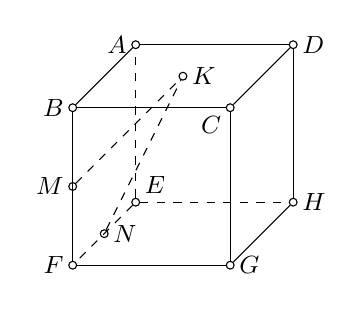
\begin{tikzpicture}
				\begin{scope}
				\small
				\tikzstyle{vnode}=[draw,circle,inner sep =1pt];
				\node[vnode] (v000) at (0,0) {};
				\node[anchor =south west] (t000) at (v000) {$E$};
				\node[vnode] (v001) at (0,2) {$$};
				\node[anchor =east] (t000) at (v001) {$A$};
				\node[vnode] (v011) at (2,2) {$$};
				\node[anchor =west] (t011) at (v011) {$D$};
				\node[vnode] (v010) at (2,0) {$$};
				\node[anchor =west] (t010) at (v010) {$H$};
				\node[vnode] (v100) at (-.8,-.8) {$$};
				\node[anchor =east] (t100) at (v100) {$F$};
				\node[vnode] (v101) at (-.8,1.2) {$$};
				\node[anchor =east] (t101) at (v101) {$B$};
				\node[vnode] (v111) at (1.2,1.2) {$$};
				\node[anchor =north east] (t111) at (v111) {$C$};
				\node[vnode] (v110) at (1.2,-0.8) {$$};
				\node[anchor =west] (t110) at (v110) {$G$};
				\node[vnode] (vK) at (.6,1.6) {$$};
				\node[anchor =west] (tK) at (vK) {$K$};
				\node[vnode] (vM) at (-.8,.2) {$$};
				\node[anchor =east] (tM) at (vM) {$M$};
				\node[vnode] (vN) at (-.4,-.4) {$$};
				\node[anchor =west] (tN) at (vN) {$N$};
				\draw[dashed] (vM) to (vK);
				\draw[dashed] (vN) to (vK);
				\foreach \i in {01,10,11}{
						\draw (v0\i) to (v1\i);
						\draw (v\i  0) to (v\i 1);
				}
				\draw[dashed] (v000) to (v100);
				\draw[dashed] (v000) to (v010);
				\draw[dashed] (v000) to (v001);
				\draw (v001) to (v011);
				\draw (v100) to (v110);
				\draw (v101) to (v111);
				\end{scope}
			\end{tikzpicture}
        \end{QBODY}
        \begin{QFROMS}
        \end{QFROMS}
        \begin{QTAGS}\QTAG{B4C1空間向量}\end{QTAGS}
        \begin{QANS}
            (1)(4)
        \end{QANS}
        \begin{QSOLLIST}
        \end{QSOLLIST}
        \begin{QEMPTYSPACE}
        \end{QEMPTYSPACE}
    \end{QUESTION}
\end{QUESTIONS}
\begin{QUESTIONS}
    \begin{QUESTION}
        \begin{ExamInfo}{098}{學測}{填充}{A}
        \end{ExamInfo}
        \begin{ExamAnsRateInfo}{76}{92}{86}{50}
        \end{ExamAnsRateInfo}
        \begin{QBODY}
			從 1 到 100 的正整數中刪去所有的質數、2 的倍數及 3 的倍數之後,剩下最大的數為 $\TCNBOX{\TCN\TCN}$ 。
        \end{QBODY}
        \begin{QFROMS}
        \end{QFROMS}
        \begin{QTAGS}\QTAG{綜合}\end{QTAGS}
        \begin{QANS}
            $95$
        \end{QANS}
        \begin{QSOLLIST}
        \end{QSOLLIST}
        \begin{QEMPTYSPACE}
        \end{QEMPTYSPACE}
    \end{QUESTION}
    \begin{QUESTION}
        \begin{ExamInfo}{098}{學測}{填充}{B}
        \end{ExamInfo}
        \begin{ExamAnsRateInfo}{31}{69}{22}{2}
        \end{ExamAnsRateInfo}
        \begin{QBODY}
			坐標平面上有四點 $O(0,0)$, $A(-3,-5)$, $B(6,0)$, $C(x,y)$。今有一質點在 $O$ 點沿 $\lvec{AO}$ 方向前進 $\lvec{AO}$ 距離後停在 $P$,再沿 $\lvec{BP}$ 方向前進 $2\overline{BP}$ 距離後停在 $Q$。 假設此質點繼續沿 $\lvec{CQ}$ 方向前進 $3\overline{CQ}$ 距離後回到原點 $O$,則 $(x,y)=\TCNBOX{\TCN\TCN,\TCN\TCN}$ 。
        \end{QBODY}
        \begin{QFROMS}
        \end{QFROMS}
        \begin{QTAGS}\QTAG{B3C3平面向量}\end{QTAGS}
        \begin{QANS}
            $(-4,20)$
        \end{QANS}
        \begin{QSOLLIST}
        \end{QSOLLIST}
        \begin{QEMPTYSPACE}
        \end{QEMPTYSPACE}
    \end{QUESTION}
    \begin{QUESTION}
        \begin{ExamInfo}{098}{學測}{填充}{C}
        \end{ExamInfo}
        \begin{ExamAnsRateInfo}{60}{92}{69}{19}
        \end{ExamAnsRateInfo}
        \begin{QBODY}
			抽獎遊戲中,參加者自箱中抽出一球,確定顏色後放回。只有抽得藍色或紅色球者可得消費劵,其金額分別為(抽得藍色球者)2000 元、(抽得紅色球者)1000 元。箱中已置有 2 顆藍色球及 5 顆 紅色球。在抽出任一球之機率相等的條件下,主辦單位希望參加者所得消費劵金額的期望值為 300 元,則主辦單位應於箱內再置入 $\TCNBOX{\TCN\TCN}$ 顆其他顏色的球。
        \end{QBODY}
        \begin{QFROMS}
        \end{QFROMS}
        \begin{QTAGS}\QTAG{B5C1機率與統計}\end{QTAGS}
        \begin{QANS}
            $23$
        \end{QANS}
        \begin{QSOLLIST}
        \end{QSOLLIST}
        \begin{QEMPTYSPACE}
        \end{QEMPTYSPACE}
    \end{QUESTION}
    \begin{QUESTION}
        \begin{ExamInfo}{098}{學測}{填充}{D}
        \end{ExamInfo}
        \begin{ExamAnsRateInfo}{39}{79}{32}{6}
        \end{ExamAnsRateInfo}
        \begin{QBODY}
			坐標平面上有兩條平行直線。它們的 $x$ 截距相差 $20$, $y$ 截距相差 $15$。則這兩條平行直線的距離為 $\TCNBOX{\TCN\TCN}$ 。
        \end{QBODY}
        \begin{QFROMS}
        \end{QFROMS}
        \begin{QTAGS}\QTAG{B3C2直線與圓}\end{QTAGS}
        \begin{QANS}
            $12$
        \end{QANS}
        \begin{QSOLLIST}
        \end{QSOLLIST}
        \begin{QEMPTYSPACE}
        \end{QEMPTYSPACE}
    \end{QUESTION}
    \begin{QUESTION}
        \begin{ExamInfo}{098}{學測}{填充}{E}
        \end{ExamInfo}
        \begin{ExamAnsRateInfo}{13}{33}{6}{0}
        \end{ExamAnsRateInfo}
        \begin{QBODY}
			假設 $\Gamma_1$ 為坐標平面上一開口向上的拋物線,其對稱軸為 $x=-\frac{3}{4}$ 且焦距(焦點到頂點的距離) 為 $\frac{1}{8}$。若 $\Gamma_1$ 與另一拋物線 $\Gamma_2 :y=x^2$ 恰交於一點,則 $\Gamma_1$ 的頂點之 $y$ 坐標為$\TCNBOX{\FR{\TCN}{\TCN}}$。(化成最簡分數)
        \end{QBODY}
        \begin{QFROMS}
        \end{QFROMS}
        \begin{QTAGS}\QTAG{B4C4二次曲線}\end{QTAGS}
        \begin{QANS}
            $\dfrac{9}{8}$
        \end{QANS}
        \begin{QSOLLIST}
        \end{QSOLLIST}
        \begin{QEMPTYSPACE}
        \end{QEMPTYSPACE}
    \end{QUESTION}
    \begin{QUESTION}
        \begin{ExamInfo}{098}{學測}{填充}{F}
        \end{ExamInfo}
        \begin{ExamAnsRateInfo}{6}{15}{2}{1}
        \end{ExamAnsRateInfo}
        \begin{QBODY}
			某公司為了響應節能減碳政策, 決定在五年後將公司該年二氧化碳排放量降為目前排放量的 $75 \%$。 公司希望每年依固定的比率(當年和前一年排放量的比) 逐年減少二氧化碳的排放量。 若要達到這項目標,則該公司每年至少要比前一年減少 $\TCNBOX{\TCN.\TCN} \%$ 的二氧化碳的排放量。 (計算到小數點後第一位, 以下四捨五入。) 
        \end{QBODY}
        \begin{QFROMS}
        \end{QFROMS}
        \begin{QTAGS}\QTAG{B1C3指對數函數}\end{QTAGS}
        \begin{QANS}
            $5.6$
        \end{QANS}
        \begin{QSOLLIST}
        \end{QSOLLIST}
        \begin{QEMPTYSPACE}
        \end{QEMPTYSPACE}
    \end{QUESTION}
    \begin{QUESTION}
        \begin{ExamInfo}{098}{學測}{填充}{G}
        \end{ExamInfo}
        \begin{ExamAnsRateInfo}{36}{80}{26}{2}
        \end{ExamAnsRateInfo}
        \begin{QBODY}
			坐標空間中 $xy$ 平面上有一正方形,其頂點為 $O(0,0,0)$, $A(8,0,0)$, $B(8,8,0)$, $C(0,8,0)$。另一點 $P$ 在 $xy$ 平面的上方,且與 $O$, $A$, $B$, $C$ 四點的距離皆等於 $6$。若 $x + by + cz = d$ 為通過 $A$, $B$, $P$ 三點的平面,則 $(b,c,d)=\TCNBOX{\TCN,\TCN,\TCN}$。
        \end{QBODY}
        \begin{QFROMS}
        \end{QFROMS}
        \begin{QTAGS}\QTAG{B4C1空間向量}\end{QTAGS}
        \begin{QANS}
            $(0,2,8)$
        \end{QANS}
        \begin{QSOLLIST}
        \end{QSOLLIST}
        \begin{QEMPTYSPACE}
        \end{QEMPTYSPACE}
    \end{QUESTION}
    \begin{QUESTION}
        \begin{ExamInfo}{098}{學測}{填充}{H}
        \end{ExamInfo}
        \begin{ExamAnsRateInfo}{36}{57}{36}{15}
        \end{ExamAnsRateInfo}
        \begin{QBODY}
			有一橢圓與一雙曲線有共同的焦點 $F_1$ 、 $F_2$ ,且雙曲線的貫軸長和橢圓的短軸長相等。設 $P$ 為此橢圓與雙曲線的一個交點,且 $\overline{PF_1} \times \overline{PF}_2 =64$ ,則 $\overline{F_1F_2} =$ 
$\TCNBOX{\TCN\TCN}$。 
        \end{QBODY}
        \begin{QFROMS}
        \end{QFROMS}
        \begin{QTAGS}\QTAG{B4C4二次曲線}\end{QTAGS}
        \begin{QANS}
            $16$
        \end{QANS}
        \begin{QSOLLIST}
        \end{QSOLLIST}
        \begin{QEMPTYSPACE}
        \end{QEMPTYSPACE}
    \end{QUESTION}
    \begin{QUESTION}
        \begin{ExamInfo}{098}{學測}{填充}{I}
        \end{ExamInfo}
        \begin{ExamAnsRateInfo}{11}{27}{5}{1}
        \end{ExamAnsRateInfo}
        \begin{QBODY}
			在 $\triangle ABC$ 中, $\overline{AB}=10$,$\overline{AC}=9$, $\cos \angle{BAC}= \frac{3}{8}$。設點 $P$, $Q$ 分別在邊 $AB$, $AC$上使得 $\triangle APQ$之面積為 $\triangle ABC$ 面積之一半,則 $\overline{PQ}$ 之最小可能值為 
			$\TCNBOX{\FR{\TCN\TCN}{\TCN}}$。
        \end{QBODY}
        \begin{QFROMS}
        \end{QFROMS}
        \begin{QTAGS}\QTAG{B3C1三角}\end{QTAGS}
        \begin{QANS}
            $\FR{15}{2}$
        \end{QANS}
        \begin{QSOLLIST}
        \end{QSOLLIST}
        \begin{QEMPTYSPACE}
        \end{QEMPTYSPACE}
    \end{QUESTION}
\end{QUESTIONS}
